\section{Results}
\label{sec:usage:results}

The specific queries given by the system and the corresponding oracle labels 
(the oracle, in this case, is the author of this work) may be seen in 
Figures~\ref{fig:usage:interesting} and \ref{fig:usage:notinteresting}. The 
system was given a budget of 15 queries.

\begin{figure}[htb]
	\begin{center}
		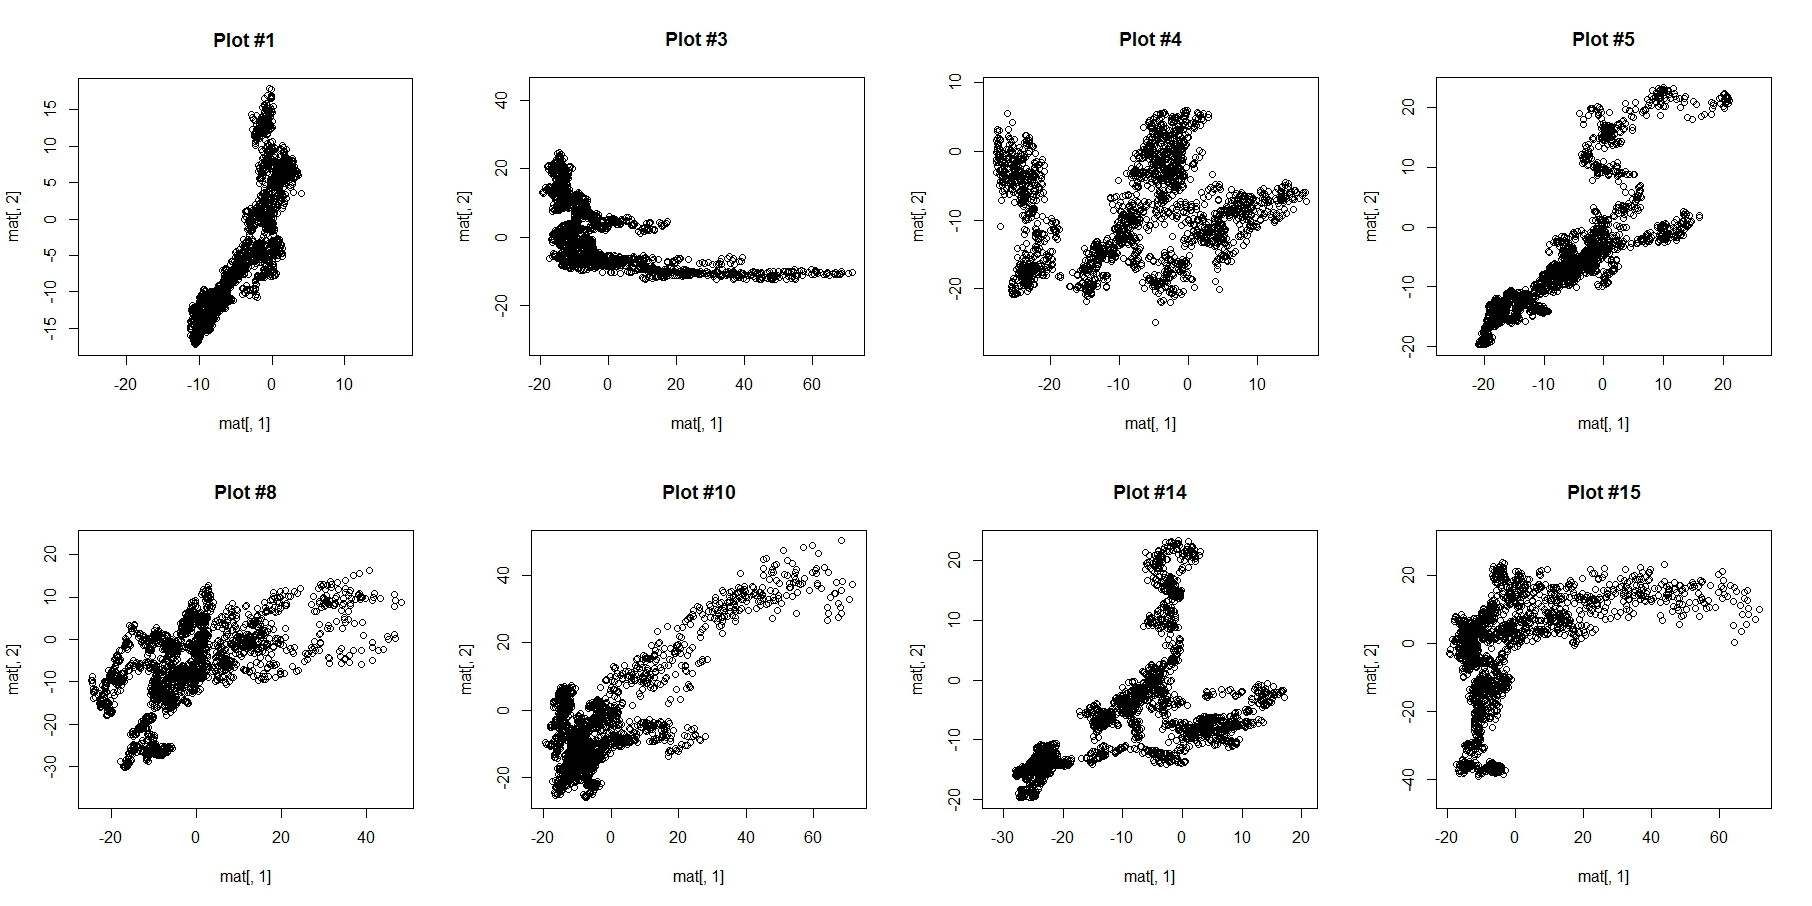
\includegraphics[width=1\linewidth]{ch-usage/figures/y_all}
		\caption[Queries which were labeled ``interesting''.]{Queries 
		which were labeled ``interesting'' (that there appears to be a visual 
		correlation).}
		\label{fig:usage:interesting}
	\end{center}
\end{figure}

\begin{figure}[H]
	\begin{center}
		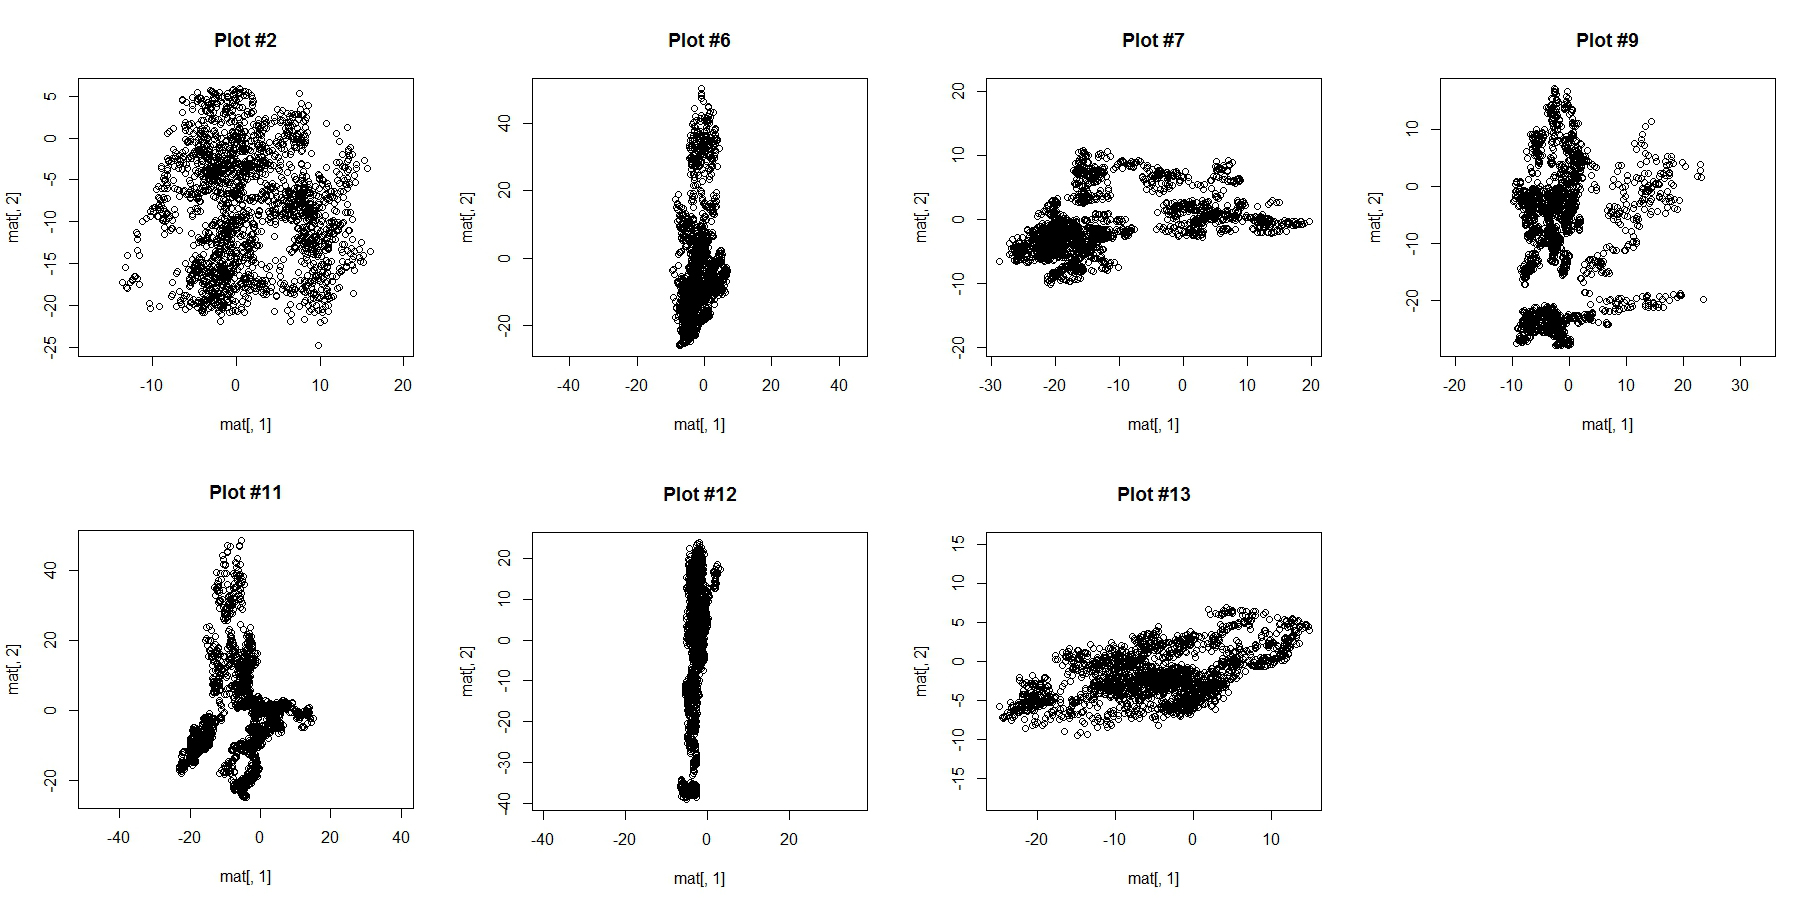
\includegraphics[width=1\linewidth]{ch-usage/figures/n_all}
		\caption[Queries which were labeled ``not interesting''.]{Queries 
			which were labeled ``not interesting'' (that there appears to be no 
			visual correlation).}
		\label{fig:usage:notinteresting}
	\end{center}
\end{figure}

It is also interesting to examine the heatmaps (which are normalized) 
corresponding to the 15 queries and the resulting decisions, which may be found 
in Figure~\ref{fig:usage:heatmaps}. A quick glance at the heatmaps reveal that 
the middle criterions are all zero. It actually turns out that these criterions 
are associated with various Pearson correlation tests (the list of associated 
criterion may be found in the comments of Figure~\ref{fig:usage:heatmaps}). 
The zero-value heatmap entry indicates that the associated $p$-values are all 
extremely low (the correlation is significantly different from zero). In 
particular, this indicates that the criterion for 9, 10, 11, 12, 13, and 14 are 
all significant. But consider the actual variable pairs associated with these 
criterion. Consider the first row, which corresponds to the first 
non-interesting plot queried (It is the first plot in 
Figure~\ref{fig:usage:notinteresting}). Specifically, the pair has a Pearson 
correlation $p$-value of 0.001728 and value of -0.069, which is close to 0 
(uncorrelated) despite the $p$-value suggesting otherwise. When looking at the 
metric numerically as the heatmap done, the natural response would be to draw 
an edge as in the heuristic given in Section~\ref{sec:intro:correlation}. 
However, looking at it visually (and even just looking at the coefficient 
without the $p$-value), it is clear that the pair is uncorrelated. How did this 
happen? Because there are 2050 samples, the variance of every pair is low, 
leading to a lower $p$-value. If the correlation graph was made solely based on 
the Pearson correlation coefficient without consideration of other factors, the 
result would have been less than ideal. This is another case demonstrating the 
usefulness of the VS.

\begin{figure}[H]
	\begin{center}
		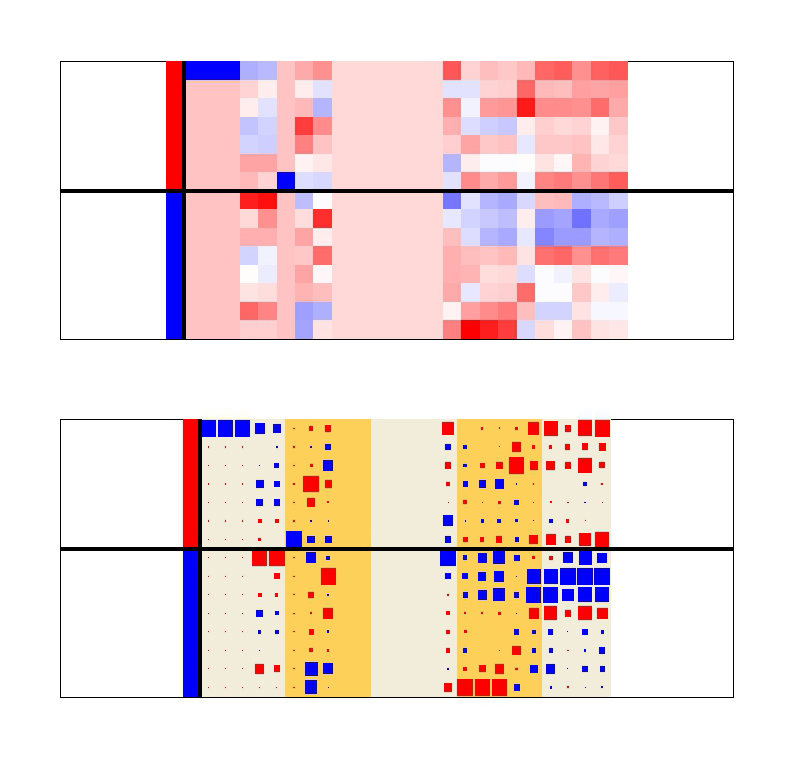
\includegraphics[width=0.8\linewidth]
		{ch-usage/figures/heatmaps}
		\caption[Normalized heatmap of the queries and given labels.] 
		{\textit{Top:} Standard heatmap of the queries and given labels 
		(normalized). 
		\textit{Bottom:} Revised heatmap (the association navigator) as 
		proposed by Buja \textit{et al.}~\cite{buja2016} (also normalized). 
		Each row corresponds to a pair that was labeled, which are ordered by 
		the oracle responses; red indicates uninteresting pairs and blue 
		indicates interesting pairs (as given by the oracle). Each column 
		corresponds to a different criterion of the associated pairwise 
		scatterplot (see Section~\ref{sec:visualizer:scatterplot}). Ordered 
		criterion list (left to right, up to down): 
		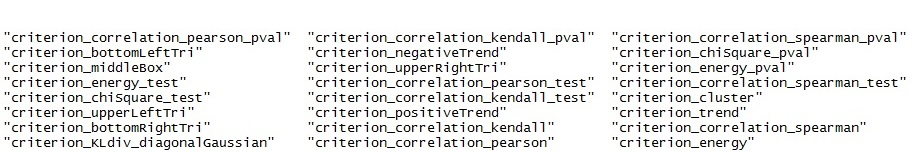
\includegraphics[width=1\linewidth]{ch-usage/figures/criterionlist}}
		\label{fig:usage:heatmaps}
	\end{center}
\end{figure}

Figure~\ref{fig:usage:hist} is a predicted probability histogram. The 
probability corresponds to correlation (interesting) or not (uninteresting) for 
100 random variable pairs. Each probability is computed using the final 
classification output of the VS. Most of the pairs fall within two bins (low 
and high probability) as shown by the two upper and lower hills in the figure, 
indicating that the classification model determined by the VS is quite 
confident regarding the labeling of most plots.

\begin{figure}[htb]
	\begin{center}
		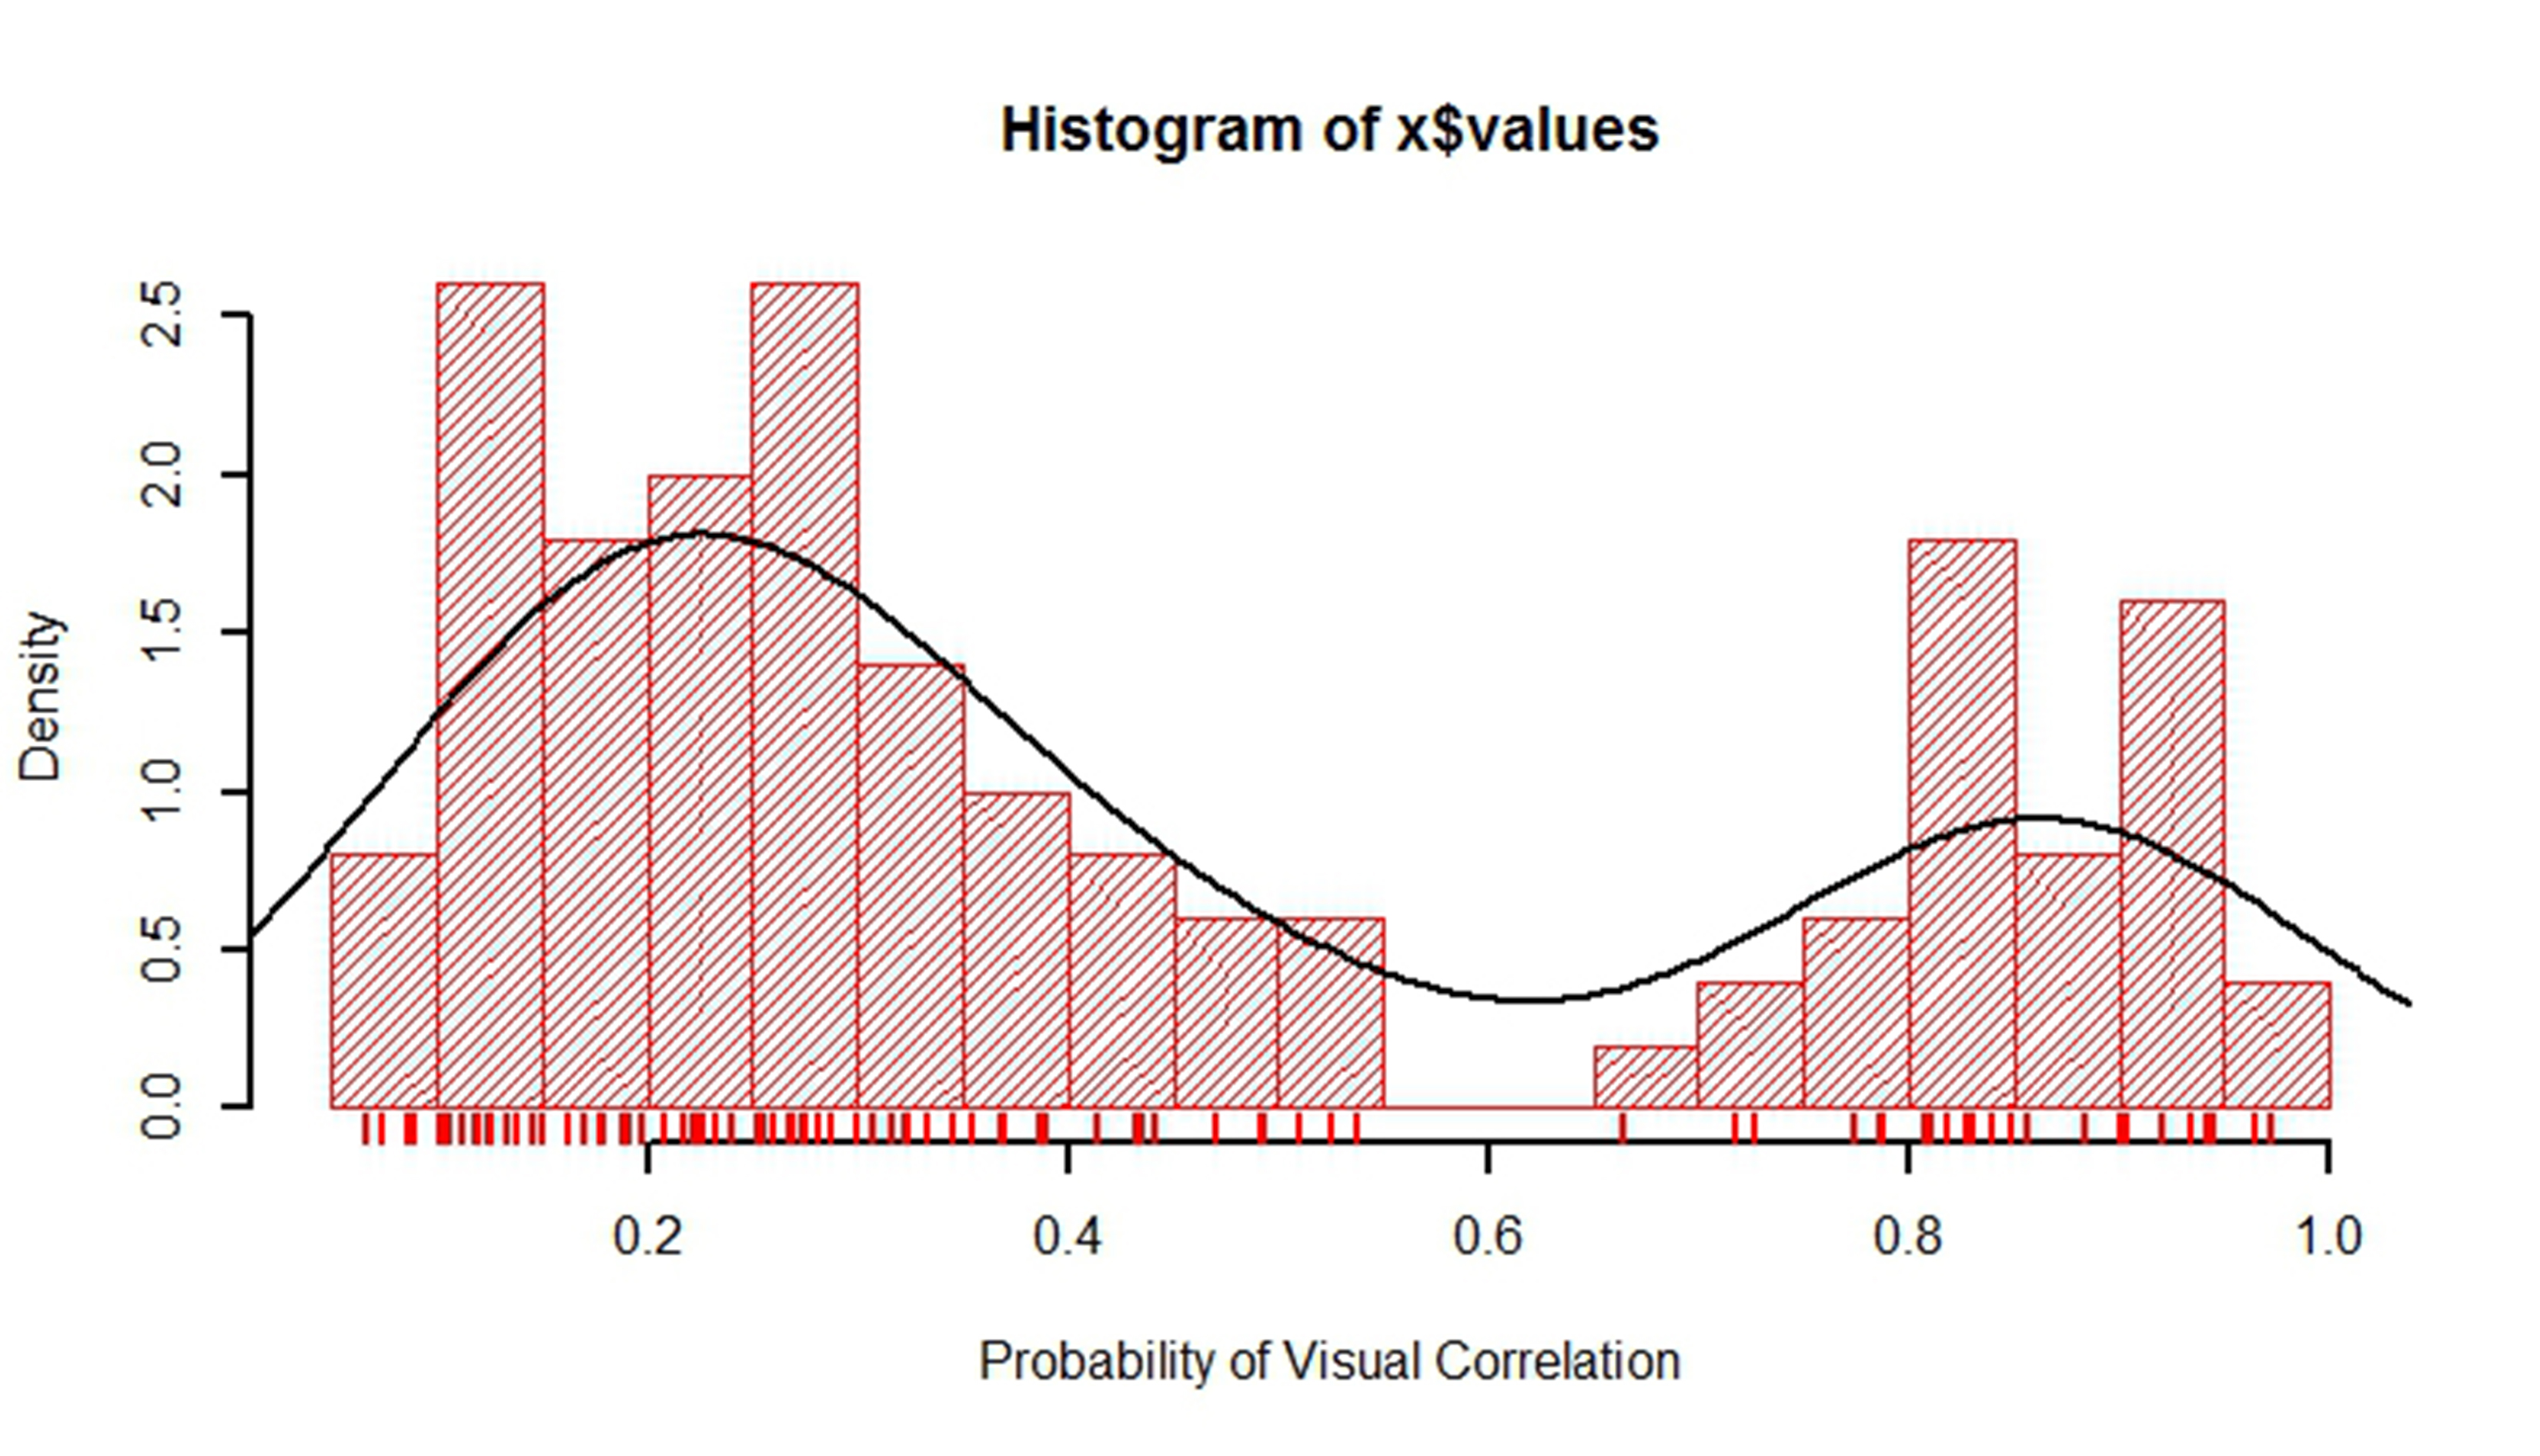
\includegraphics[width=1\linewidth]
		{ch-usage/figures/predicted_probability_histogram}
		\caption[Histogram of predicted probabilities.]{The histogram shows the 
		predicted probabilities for each of 100 random variable pairs. The 
		probability corresponds to the probability of a plot being 
		``interesting'' or ``not interesting''.}
		\label{fig:usage:hist}
	\end{center}
\end{figure}

\newpage
The final resulting visual graph is plotted in Figure~\ref{fig:usage:visg}. 

\begin{figure}[H]
	\begin{center}
		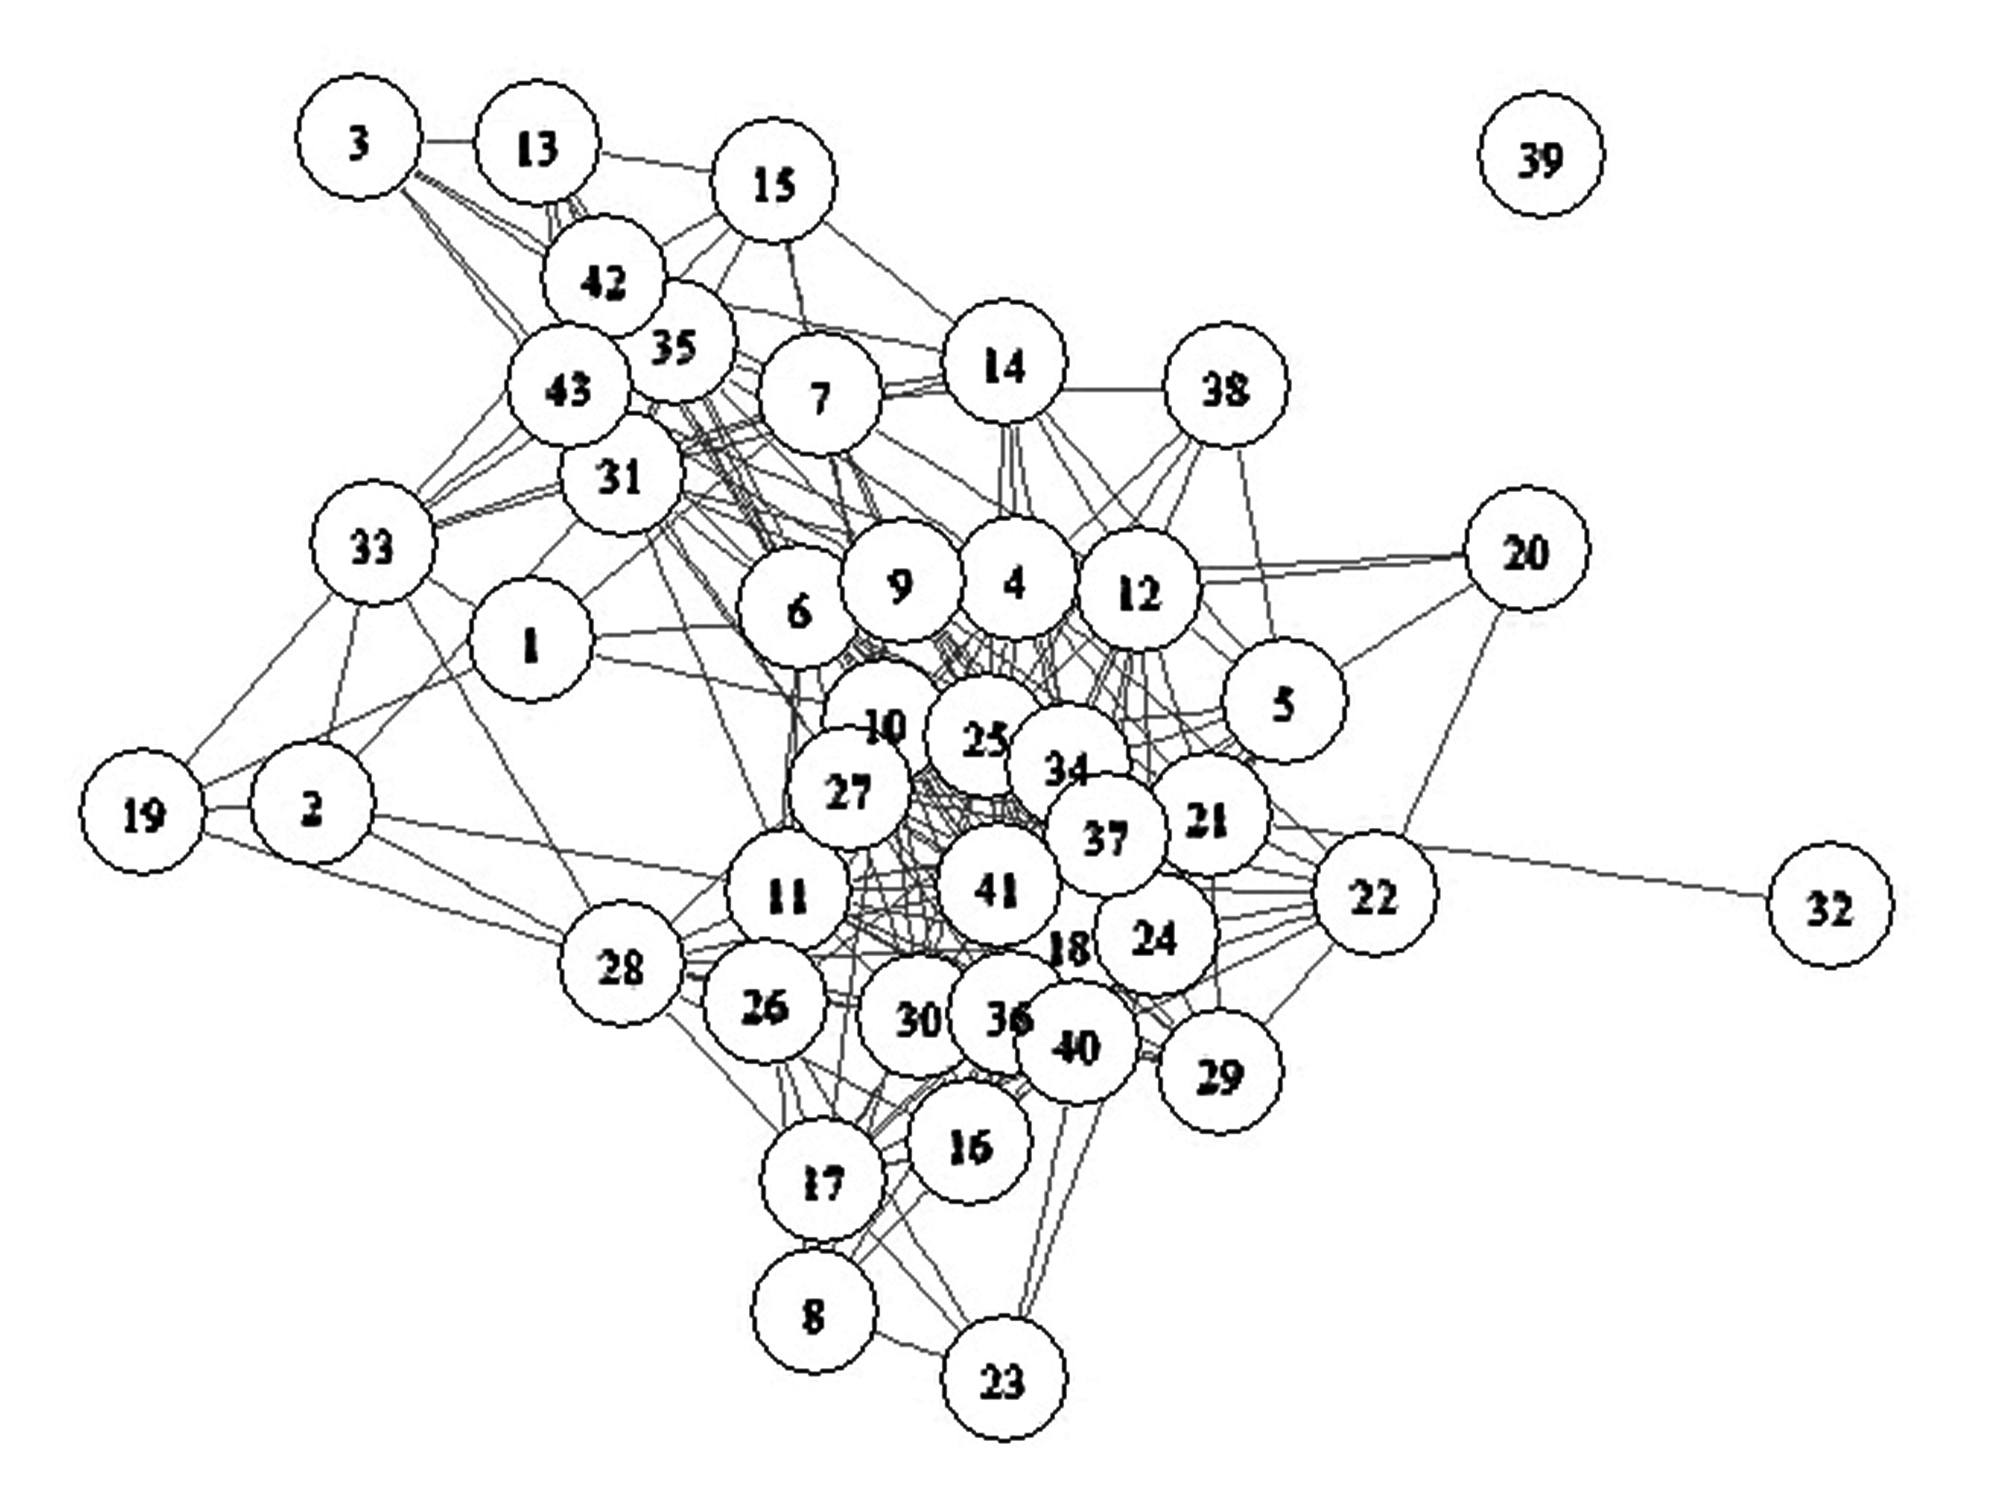
\includegraphics[width=0.5\linewidth]
		{ch-usage/figures/visgraph}
		\caption[Visual graph output from the visualization system.]{Visual 
		graph output from the visualization system.}
		\label{fig:usage:visg}
	\end{center}
\end{figure}

The graph comparison determined that the \textbf{distance correlation graph} is 
closest to the visual correlation graph. 
The computed graph difference in Table~\ref{tab:usage:graphdiff}.
As a sanity check, this 
matches our intuition as distance correlation is the most nuanced of the four 
correlation coefficients, and a value of 0 actually indicates independence. The 
resulting portfolios selected by the procedure in 
Section~\ref{sec:usage:stockselection} for each correlation graph are 
summarized in Table~\ref{tab:usage:returns}.

Finally, the the ``buy and hold'' performance (yearly returns) and cumulative 
sum of returns are plotted for the S\&P 500 (the CONTROL), 
the portfolios created from the various numerical correlation graphs 
including  $G^*$ (which corresponds to distance correlation), 
and the portfolio created from the final visual correlation graph 
$G^{\text{vis}}$ may be found in Figure~\ref{fig:usage:returns}. The associated 
data may be found in Table~\ref{tab:usage:returns}. Note 
that the ``yearly'' returns for 2006 and 2014 are low because the data begins 
on 3/14/2006 and ends on 5/13/2004; as such, those returns do not reflect a 
full year of data. Our focus is mostly diverted to the full years in between 
and especially the performance during the financial crisis. 

The portfolio $P^*$, constructed from the numerical distance correlation graph 
$G^*$ which was selected due to its similarity to $G$, performs the strongest 
by far. $P^*$ consistently posts the highest returns year after year. Though it 
doesn't seem like much in the first plot of yearly returns, the differences 
really add up as can be seen in the second plot of the cumulative sum. Further 
consider the financial crisis; $P^*$ has the least negative returns of 2008. 
This indicates that the visual graph is capturing the independence and 
dependence among various stocks properly, which translates into the selection 
of $G^*$ and, subsequently, $P^*$, a portfolio that is well balanced and 
captures the spirit of the ``buy and hold'' model described in 
Section~\ref{sec:intro:finance}.

%$P^{\text{vis}}$ catches up after a mediocre beginning, and there are other 
%interesting things to note about its performance that makes it difficult to 
%definitively say which portfolio is ``better''. Consider the financial crisis; 
%while the positive returns and recovery of $P^{\text{vis}}$ are muted, it has 
%the most significant least negative returns of 2008. This is an indication
%that the visual graph is capturing precisely what we wish for it to capture 
%(independence and dependence among various stocks), which is translating into 
%a portfolio that is well balanced and captures the spirit of the ``buy and 
%hold'' model described in Section~\ref{sec:intro:finance}. The persistence in 
%holding the portfolio ends up paying off returns rapid increase until the 
%portfolio is the top performer in 2011 and beyond.

As noted earlier in Section~\ref{sec:usage:stockselection}, the proposed stock 
selection strategy is simple, but every selected portfolio has outperformed the 
S\&P500, suggesting that an even more sophisticated selection procedure would 
yield even more fruitful returns.


\begin{landscape}
	\tablespacing
	\begin{longtable}{p{0.1\linewidth}p{0.15\linewidth}p{0.13\linewidth}
			p{0.13\linewidth}p{0.13\linewidth}p{0.13\linewidth} }
		
		% First page heading
		\caption[Computed differences between the visual correlation graph and 
		various numerical correlation graphs.]{Computed differences between the 
		visual correlation graph and various numerical correlation graphs. See 
		Section~\ref{sec:gc:methods} for details on each graph summarization 
		metric.} 
		\label{tab:usage:graphdiff}\\
		\toprule
		\textbf{Graph Type} & \textbf{Centrality \newline (degree)} & 
		\textbf{Centrality \newline (closeness)} & 
		\textbf{Centrality \newline (betweenness)} & 
		\textbf{Assortativity} & \textbf{Distance \newline matrix} \\
		\midrule
		\endfirsthead
		
		% Last page footer
		\bottomrule
		\endlastfoot

		Pearson's & 0.0034 & 0.0119 & 0.0032 & 0.061 & 0.0313\\
		
		Spearman's & 0.0052 & 0.0079 & 0.0032 & 0.0773 & 0.029\\
		
		Kendall's & 0.0002 & 0.019 & 0.0024 & 0.0559 & 0.0253\\
		
		Distance & 0.0018 & 0.0276 & 0.0012 & 0.0465 & 0.0206\\
		
		\midrule
		
		& \textbf{Community\newline (random walk)} & 
		\textbf{Community \newline (infomap)} & 
		\textbf{Community \newline (betweenness)} & 
		\textbf{Edge\newline connectivity} & 
		\textbf{Edge density \newline histogram} \\
		 	
		\midrule
		
		Pearson's & 0.7602 & 0.5039 & 0.6488 & 1 & 0.6014\\
		
		Spearman's & 0.8478 & 0.5039 & 0.6948 & 1 & 0.5625\\
		
		Kendall's & 1 & 0.5039 & 0.7284 & 1 & 0.4413\\
		
		Distance & 0.253 & 0.5039 & 0.5437 & 1 & 0.2455\\
		
	\end{longtable}
	\bodyspacing
\end{landscape}





\begin{figure}[htb]
	\begin{center}
		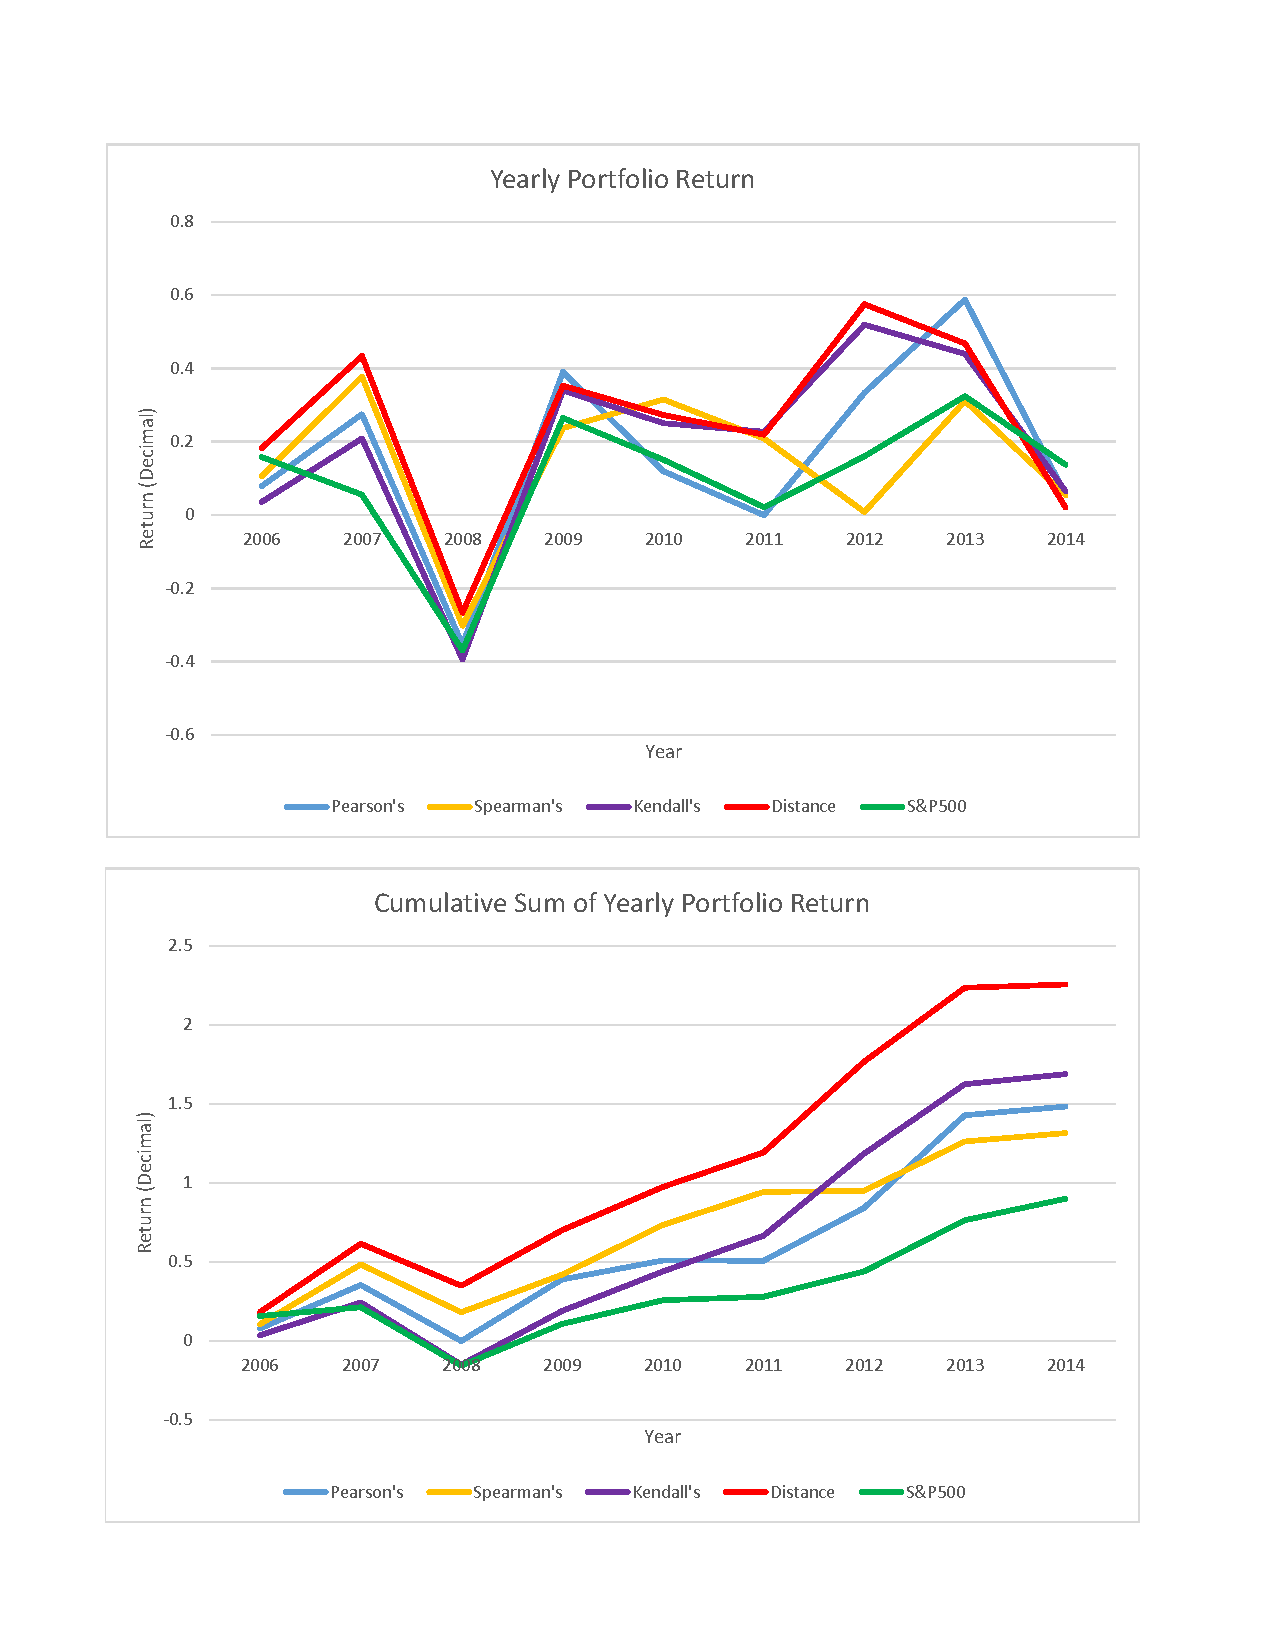
\includegraphics[width=1\linewidth]
		{ch-usage/figures/Results_YearlyReturns.pdf}
		\caption[Yearly and cumulative performance of the selected portfolios 
		and the S\&P500.]{Yearly and cumulative performance of the selected 
		portfolios and the S\&P500. Note that the ``yearly'' returns for 2006 
		and 2014 are low because the data begins on 3/14/2006 and ends on 
		5/13/2004; as such, those returns do not reflect a full year of data. 
		The associated data may be found in Table~\ref{tab:usage:returns}.}
		\label{fig:usage:returns}
	\end{center}
\end{figure}




\begin{landscape}
\tablespacing
\begin{longtable}{p{0.15\linewidth}p{0.15\linewidth}p{0.05\linewidth}
p{0.05\linewidth}p{0.05\linewidth}p{0.05\linewidth} 
p{0.05\linewidth}p{0.05\linewidth}p{0.05\linewidth} 
p{0.05\linewidth}p{0.05\linewidth}p{0.05\linewidth} 
p{0.05\linewidth}}
	
	% First page heading
	\caption[Yearly portfolio returns for each correlation graph.]{Yearly 
	portfolio returns for each correlation graph (decimal).} 
	\label{tab:usage:returns}\\
	\toprule
	\textbf{Graph Type} & \textbf{Portfolio} & \textbf{2006} 
	& \textbf{2007} & \textbf{2008} & \textbf{2009} & 
	\textbf{2010} & \textbf{2011} & \textbf{2012} & 
	\textbf{2013} & \textbf{2014} \\
	\midrule
	\endfirsthead
	
	% Future page heading
	\caption[]{(continued)}\\
	\toprule
	\textbf{Graph Type} & \textbf{Portfolio} & \textbf{2006} 
	& \textbf{2007} & \textbf{2008} & \textbf{2009} & 
	\textbf{2010} & \textbf{2011} & \textbf{2012} & 
	\textbf{2013} & \textbf{2014} \\
	\midrule
	\endhead
	
	% Page footer
	\midrule
	\multicolumn{11}{r}{(Continued on next page)}\\
	\endfoot
	
	% Last page footer
	\bottomrule
	\endlastfoot

	S\&P500 \newline (CONTROL) & \textbf{Total} & 
	0.158&0.055&-0.37&0.265&0.151&0.021&0.16&0.324&0.137\\
	
	\cmidrule[0.1pt](l{0.5em}r{0.5em}){1-11}	
	
	Pearson's &CI&0.041&0.226&-0.686&1.099&0.041&0.147&0.274&0.637&0.011\\
	&GILD&0.056&0.417&0.111&-0.154&-0.162&0.129&0.795&1.045&0.069\\
	&SYK&0.15&0.362&-0.46&0.267&0.079&-0.061&0.121&0.393&0.073\\
	&TMO&0.276&0.274&-0.409&0.4&0.161&-0.188&0.432&0.758&0.057\\
	&VAR&-0.131&0.096&-0.328&0.337&0.479&-0.031&0.046&0.106&0.064\\
	&\textbf{Total}&0.078&0.275&-0.354&0.39&0.119&-0.001&0.333&0.588&0.055\\
	
	\cmidrule[0.1pt](l{0.5em}r{0.5em}){1-11}	
	
	Spearman's &HUM&0.122&0.362&-0.505&0.177&0.247&0.615&-0.206&0.523&0.184\\
	&LH&0.291&0.028&-0.147&0.162&0.175&-0.022&0.008&0.055&0.092\\
	&PRGO&0.096&1.041&-0.072&0.243&0.597&0.542&0.073&0.479&-0.144\\
	&SYK&0.15&0.362&-0.46&0.267&0.079&-0.061&0.121&0.393&0.073\\
	&VAR&-0.131&0.096&-0.328&0.337&0.479&-0.031&0.046&0.106&0.064\\
	&\textbf{Total}&0.106&0.378&-0.302&0.237&0.315&0.208&0.008&0.311&0.054\\
	
	\cmidrule[0.1pt](l{0.5em}r{0.5em}){1-11}	
	
	Kendall's&MCK&-0.039&0.297&-0.404&0.63&0.138&0.118&0.256&0.676&0.117\\
	&REGN&0.231&0.203&-0.24&0.317&0.358&0.688&2.086&0.609&0.03\\
	&SYK&0.15&0.362&-0.46&0.267&0.079&-0.061&0.121&0.393&0.073\\
	&UNH&-0.035&0.084&-0.543&0.148&0.199&0.422&0.086&0.41&0.04\\
	&VAR&-0.131&0.096&-0.328&0.337&0.479&-0.031&0.046&0.106&0.064\\
	&\textbf{Total}&0.035&0.209&-0.395&0.34&0.25&0.227&0.519&0.439&0.065\\
	
	%\cmidrule[0.1pt](l{0.5em}r{0.5em}){1-11}			
	\newpage
	
	Distance&JNJ&0.137&0.036&-0.078&0.113&-0.006&0.099&0.108&0.346&0.111\\
	(Most similar to 
	&PRGO&0.096&1.041&-0.072&0.243&0.597&0.542&0.073&0.479&-0.144\\
	visual graph)&REGN&0.231&0.203&-0.24&0.317&0.358&0.688&2.086&0.609&0.03\\
	&TMO&0.276&0.274&-0.409&0.4&0.161&-0.188&0.432&0.758&0.057\\
	&WAT&0.169&0.615&-0.536&0.691&0.254&-0.047&0.177&0.148&0.048\\
	&\textbf{Total}&0.182&0.434&-0.267&0.353&0.273&0.219&0.575&0.468&0.021\\
	
\end{longtable}
\bodyspacing
\end{landscape}